% !TeX root = it-governance-risk-compliance.tex
% !TeX encoding = UTF-8
\chapter{Merancang Sistem Tata Kelola Target}

\section*{Tujuan Pembelajaran}
\begin{itemize}
  \item Merancang struktur tata kelola target, termasuk forum keputusan, peran kunci, dan
  matriks RACI.
  \item Menetapkan target kapabilitas COBIT dan profil target NIST CSF yang selaras dengan
  \textit{risk appetite}.
  \item Mengaitkan praktik ITIL 4 dengan objektif manajemen COBIT untuk menjalankan layanan TI
  sehari-hari.
\end{itemize}

\section{Pendahuluan}

Semua pimpinan Medikara menyetujui strategi Satu Pasien, Satu Rekam Medis. Perselisihan baru
muncul ketika keputusan nyata datang. Misalkan mitra asuransi meminta integrasi untuk 6.000
klaim per bulan. Tim platform teknologi informasi (TI) ingin segera membuka data, pemilik
layanan khawatir terhadap gangguan, dan fungsi hukum meminta pembatasan tujuan. Usulan itu
berpindah antarforum selama 4 bulan. Selama itu 24.000 klaim tetap diproses manual, dan belum
ada yang dapat menyebut siapa pemutusnya.

Medikara membutuhkan tata kelola yang menjawab dua pertanyaan: siapa menyetujui pembukaan data
kepada mitra, dan siapa memegang akuntabilitas atas rekam medis terpadu. Bab 4 sampai Bab 7
sudah memberi bahannya, yaitu enam objektif awal, 12 skenario risiko, 14 baris profil keamanan,
dan 13 celah. Bab ini mengubah bahan itu menjadi model tata kelola target untuk tonggak C3
capstone. Model tersebut harus menutup celah C2, sepadan dengan kemampuan organisasi, dan
terhubung dengan rancangan tiga mata kuliah lain.

Bab ini memakai panduan desain Control Objectives for Information and Related Technologies
(COBIT) 2019 untuk menetapkan target, National Institute of Standards and Technology
Cybersecurity Framework (NIST CSF) 2.0 untuk profil target keamanan, dan Information Technology
Infrastructure Library (ITIL) 4 untuk praktik layanan. ISO/IEC 38500:2024 dan Three Lines Model
dari The Institute of Internal Auditors (IIA) menjadi pegangan pembagian peran. ISO adalah
International Organization for Standardization, dan IEC adalah International Electrotechnical
Commission. Naskah COBIT, ITIL, dan ISO berbayar, sehingga rinciannya ditulis ringkas dan perlu
dicocokkan ke naskah berlisensi sebelum dipakai untuk penilaian formal. Publikasi NIST terbuka.
Pilihan target dan angka biaya merupakan skenario pembelajaran
\cite{cobit2019-design,nistcsf2,itil4,iso38500-2024,iia-tlm2026}.

\IfFileExists{../figures/ch08-diagram-konsep.png}{%

Gambar \ref{fig:ch08-ilustrasi-bab} merangkum hubungan komponen dan konsep utama bab ini.
\begin{figure}[!htb]
  \centering
  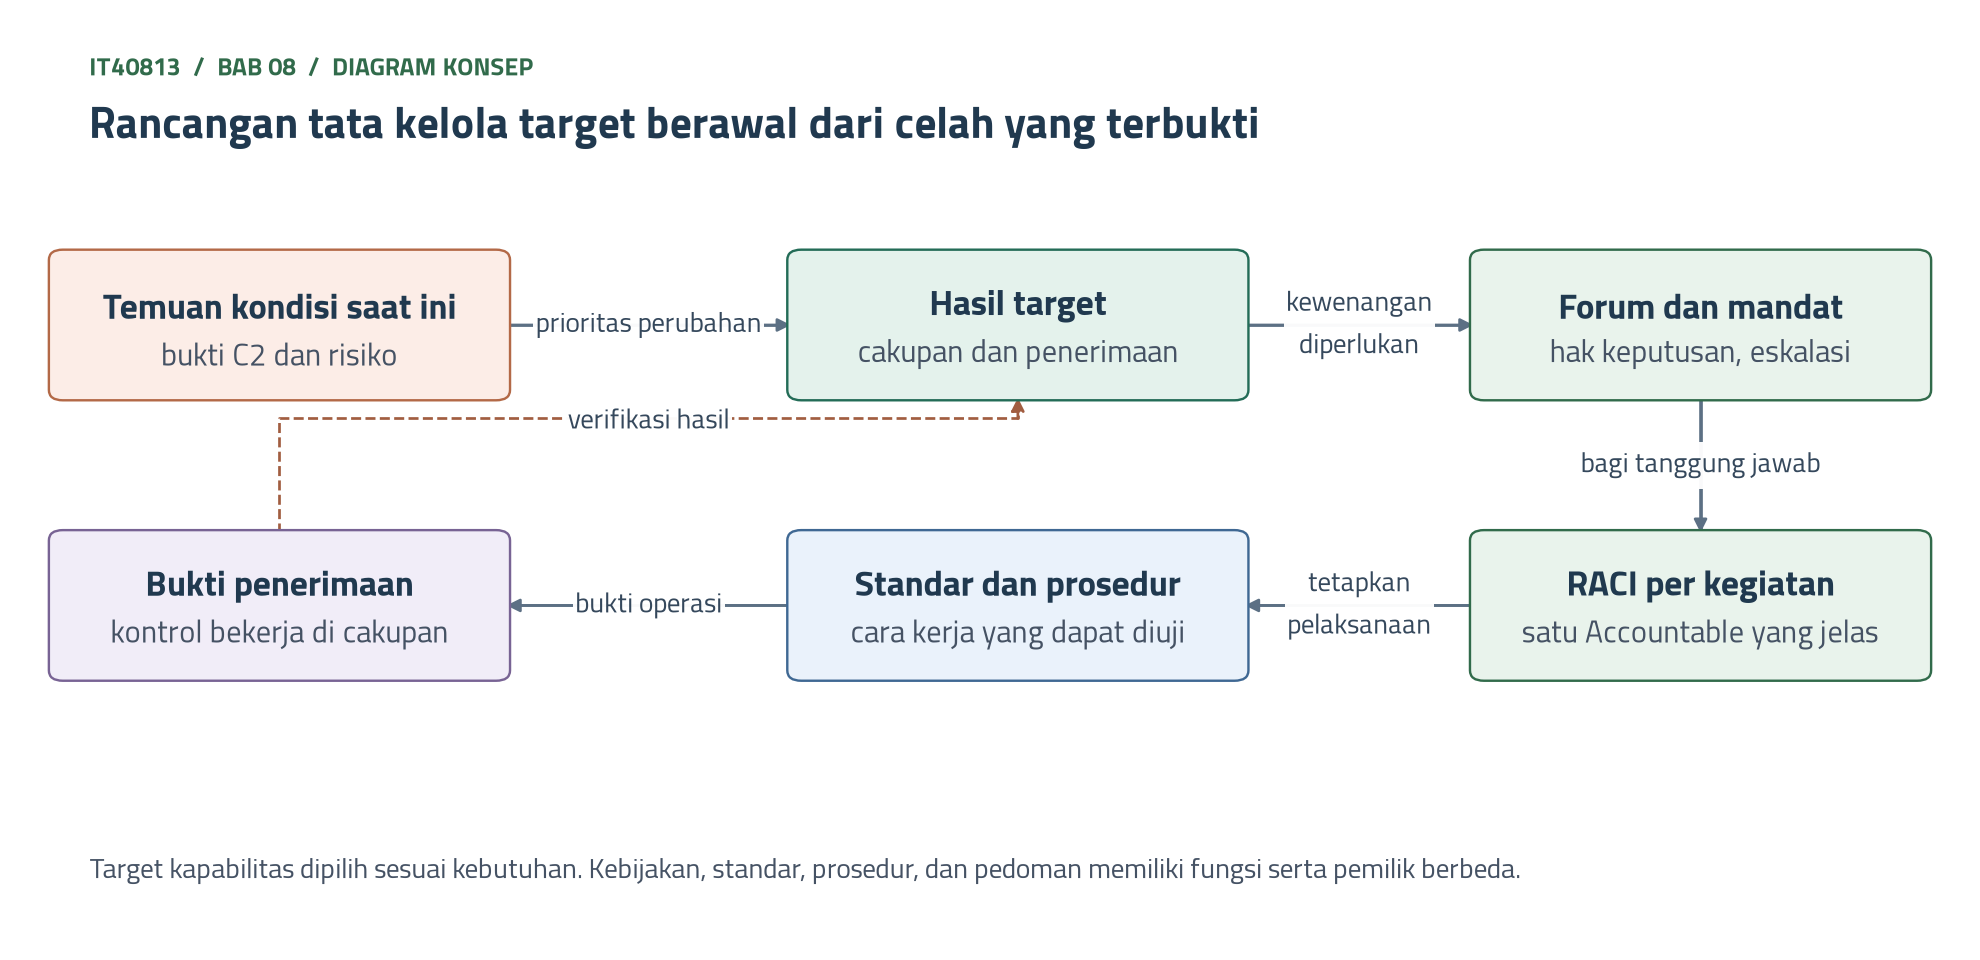
\includegraphics[width=\textwidth]{../figures/ch08-diagram-konsep.png}
  \caption{Rancangan tata kelola target berawal dari celah yang terbukti}
  \label{fig:ch08-ilustrasi-bab}
\end{figure}
}{}

\section{Dari Temuan C2 ke Keputusan Target}

\subsection*{Empat tahap panduan desain}

Desain target menjelaskan hasil yang ingin dicapai dan cara mempertanggungjawabkannya. Panduan
desain COBIT 2019 memuat empat tahap: memahami konteks dan strategi, menetapkan cakupan awal,
menyempurnakan cakupan, lalu menyelesaikan konflik dan menyimpulkan rancangan
\cite{c08-isaca-press}. Tahap akhir memberi tiap objektif terpilih tingkat kapabilitas target
\cite{c04-kapabilitas}. Rancangan ini berulang. Bila konteks, strategi, atau faktor desain
berubah, rancangan ditinjau lagi \cite{c08-grijp2019}.

Analogi renovasi rumah memperjelas urutannya. Penghuni menetapkan kebutuhan, memeriksa kondisi,
memilih perubahan, lalu menyepakati rancangan serta biaya. Mengganti seluruh bagian dengan bahan
termahal tidak selalu menyelesaikan masalah utama.

Dua contoh menghubungkan target dengan bukti:
\begin{enumerate}
  \item Misalkan AC-01 baru punya bukti pada 1 dari 5 rumah sakit, atau 12 dari 60 catatan
  peninjauan per tahun. Target awal adalah peninjauan bulanan dengan bukti pencabutan pada
  seluruh lokasi, yaitu 60 dari 60 catatan, bukan langsung otomatisasi penuh. Perluasan itu
  berbiaya Rp60 juta per tahun pada hitungan Bab 5.
  \item Misalkan laporan 18 klinik tidak konsisten karena definisi indikator berbeda. Bila tiap
  klinik memerlukan 2 jam rekonsiliasi per bulan, pekerjaannya 432 jam per tahun, atau Rp25,92
  juta pada tarif Rp60.000 per jam dari Bab 7. Target menetapkan pemilik definisi dan aturan
  rekonsiliasi. Mengganti aplikasi lembar kerja tanpa definisi yang sama hanya menghasilkan
  angka berbeda lebih cepat.
\end{enumerate}

Gambar~\ref{fig:ch08-desain} menempatkan keempat tahap pada urutan capstone. Bab 4 memakai
faktor desain untuk memilih enam objektif awal, tetapi berhenti pada kondisi saat ini. Bab ini
mengerjakan tahap keempat.

\begin{figure}[!htb]
  \centering
  \begin{tikzpicture}[
  font=\scriptsize,
  tahap/.style={draw, rounded corners, align=center, text width=2.4cm,
    minimum height=1.05cm, fill=blue!8},
  capstone/.style={draw, rounded corners, align=center, minimum height=1.2cm},
  panah/.style={-{Stealth[length=2mm]}, thick},
  tautan/.style={dashed, -{Stealth[length=2mm]}}]
  \node[anchor=south west, font=\scriptsize\bfseries] at (-1.3,0.55)
    {Panduan desain COBIT 2019};
  \node[tahap] (t1) at (0,0) {1. Konteks\\dan strategi};
  \node[tahap] (t2) at (3,0) {2. Cakupan awal};
  \node[tahap] (t3) at (6,0) {3. Penyempurnaan\\cakupan};
  \node[tahap, fill=orange!12] (t4) at (9,0) {4. Kesimpulan\\rancangan};
  \draw[panah] (t1) -- (t2);
  \draw[panah] (t2) -- (t3);
  \draw[panah] (t3) -- (t4);
  \node[anchor=south west, font=\scriptsize\bfseries] at (0.15,-1.3) {Capstone Medikara};
  \node[capstone, fill=blue!8, text width=2.4cm] (c1) at (0,-2.2)
    {C1: strategi,\\hak keputusan,\\kewajiban};
  \node[capstone, fill=blue!8, text width=5.4cm] (c2) at (4.5,-2.2)
    {C2: Bab 4 memilih 6 objektif awal;\\Bab 5 sampai 7: risiko dan 13 celah};
  \node[capstone, fill=green!10, text width=2.4cm] (c3) at (9,-2.2)
    {C3: target, forum,\\RACI, kebijakan};
  \draw[tautan] (t1.south) -- (c1.north);
  \draw[tautan] (t2.south) -- (t2.south |- c2.north);
  \draw[tautan] (t3.south) -- (t3.south |- c2.north);
  \draw[tautan] (t4.south) -- (c3.north);
\end{tikzpicture}

  \caption{Empat tahap panduan desain dan penerapannya pada capstone}
  \label{fig:ch08-desain}
\end{figure}

Diagram konsep pada awal bab meringkas urutan kerja yang sama. Temuan kondisi saat ini memberi
prioritas perubahan. Prioritas menjadi hasil target beserta cakupan dan syarat penerimaannya.
Hasil target menentukan kewenangan yang diperlukan, sehingga forum dan mandat dirancang
sesudahnya. Forum membagi tanggung jawab ke dalam matriks \textit{Responsible, Accountable,
Consulted, Informed} (RACI) per kegiatan. RACI menetapkan pelaksanaan lewat standar dan
prosedur. Standar dan prosedur menghasilkan bukti operasi, lalu bukti penerimaan memverifikasi
hasil target. Seksi berikut mengikuti urutan itu.

\subsection*{Dari 13 celah menjadi empat paket}

Pertanyaan kemudian muncul: bagaimana memilih target ketika anggaran terbatas? Tim membandingkan
dampak celah terhadap batas risiko Bab 5, kewajiban hukum, ketergantungan, dan bukti hasil. Tim
juga mencatat inisiatif yang ditunda serta akibat penundaannya.

Bab 6 menghasilkan G-01 sampai G-06, dan Bab 7 menghasilkan CP-01 sampai CP-07, sehingga ada 13
celah. Masing-masing bab memilih tiga prioritas, yaitu G-01, G-03, dan G-05, serta CP-04, CP-01,
dan CP-05. Enam prioritas itu saling bertaut. CP-01 dan G-01 sama-sama menyentuh akun vendor.
CP-04 dan G-05 sama-sama menyentuh insiden bersama vendor. Tabel~\ref{tab:ch08-paket}
menyatukannya menjadi empat paket target. Seluruh target merupakan pengandaian.

\begin{table}[!htb]
  \centering\small
  \caption{Empat paket target dari celah prioritas C2 (misalkan)}\label{tab:ch08-paket}
  \begin{tabularx}{\textwidth}{|>{\raggedright\arraybackslash}p{0.13\textwidth}|>{\raggedright\arraybackslash}p{0.09\textwidth}|>{\raggedright\arraybackslash}p{0.12\textwidth}|>{\raggedright\arraybackslash}X|>{\raggedright\arraybackslash}X|}
    \hline
    \textbf{Paket} & \textbf{Celah} & \textbf{Risiko, kewajiban} & \textbf{Hasil target} &
    \textbf{Bukti penerimaan} \\ \hline
    A. Akses vendor & G-01, CP-01 & R-01, K-01, K-05 & Peninjauan bulanan pada 5 rumah sakit;
    perjanjian vendor lengkap & 120 dari 120 akun cocok; 60 dari 60 catatan AC-01; 11 dari 11
    butir perjanjian \\ \hline
    B. Pemulihan & G-03 & R-05, K-02 & Uji pemulihan terjadwal pada 36 fasilitas & 144 uji per
    tahun; hasil disahkan pemilik layanan \\ \hline
    C. Insiden dan pemberitahuan & G-05, CP-04 & R-01, R-12, K-04, K-05 & Prosedur bersama
    vendor dilatih & 2 latihan per tahun; laporan vendor dalam 12 jam; naskah siap sebelum jam
    ke-60 \\ \hline
    D. Jejak aktivitas & CP-05, G-02 & R-01, R-12, K-01 & Catatan rinci disimpan 90 hari dan
    ditinjau & Uji telusur satu rekam; 247 dari 260 tinjauan mingguan \\ \hline
  \end{tabularx}
\end{table}

Tujuh celah sisanya tidak dihapus. G-02 ikut Paket D. CP-06 selesai lewat rancangan peran pada
bab ini. CP-03 menjadi syarat alur berbagi data asuransi. G-04, G-06, CP-02, dan CP-07 tetap
tercatat dengan pemiliknya dan masuk gelombang kedua. R-11 tetap berada pada jalur pimpinan
klinis dengan direktur pelayanan sebagai pemilik risiko, seperti Bab 5.

Keputusan ini punya dua konsekuensi yang dapat dihitung. Pertama, beban kerjanya terukur. Bab 6
menghitung 576 jam per tahun untuk G-01 dan G-03. Bab 7 menghitung 96 jam per tahun untuk
latihan pemberitahuan. Misalkan satu tinjauan catatan aktivitas memerlukan 2 jam, sehingga 260
tinjauan memakan 520 jam. Totalnya 1.192 jam per tahun, atau sekitar 0,62 orang penuh waktu pada
1.920 jam kerja per tahun. Dengan tarif Rp60.000 per jam, nilainya Rp71,52 juta. Angka itu hanya
waktu staf, dan sebagian sudah termasuk dalam Rp60 juta untuk AC-01 pada Bab 5, sehingga kedua
angka tidak dijumlahkan begitu saja. Kedua, penundaan punya akibat. G-04 dan G-06 berkaitan
dengan R-02 berskor 12, sehingga R-02 tetap terbuka selama gelombang pertama. Pemilik Sistem
Informasi Manajemen Rumah Sakit (SIMRS) perlu mengetahui penundaan itu dan menyetujuinya secara
tertulis.

\section{Menetapkan Target Kapabilitas COBIT}

\subsection*{Target tidak sama dengan tingkat tertinggi}

Target kapabilitas menyatakan tingkat yang dituju untuk proses pada objektif terpilih. Bab 4
sudah menjelaskan maknanya. Tingkat 2 mencapai tujuan lewat aktivitas dasar yang lengkap.
Tingkat 3 memakai cara kerja dan aset organisasi. Tingkat 4 mengukur kinerja secara kuantitatif.
Tingkat 5 memakai pengukuran untuk perbaikan berkelanjutan \cite{c04-kapabilitas}. Tingkat lebih
tinggi menuntut lebih banyak aset, pengukuran, dan orang, sehingga tingkat tertinggi bukan
tujuan yang berlaku untuk seluruh proses.

Menurut Souza Neto dan rekan, contoh pada panduan desain memberi tingkat 4 untuk skor 75 atau
lebih, tingkat 3 untuk skor 50 atau lebih, tingkat 2 untuk skor 25 atau lebih, dan tingkat 1
untuk sisanya. Skor 75 pada contoh itu berarti kepentingan objektif sedikitnya 75 persen lebih
tinggi daripada situasi pembanding. Mereka mengkritik satu akibatnya: semua proses pada objektif
berskor sama menerima satu tingkat yang sama \cite{c04-kapabilitas}.

Analogi kendaraan rumah sakit menjelaskan pilihan itu. Ambulans diperiksa setiap hari dengan
catatan terukur. Mobil pengantar berkas cukup diservis berkala. Menyamakan keduanya menghabiskan
biaya tanpa menaikkan keselamatan.

Dua contoh memperlihatkan kesalahan yang sering muncul:
\begin{enumerate}
  \item Misalkan analis mengubah skor lokal DSS05 pada Bab 4, yaitu 12 dari 15, menjadi 80
  persen, lalu memakai ambang 75 sehingga DSS05 mendapat tingkat 4. Hitungan itu salah skala.
  Skor lokal Bab 4 adalah pengandaian dengan nilai maksimum 15. Ambang 75 berasal dari skor
  kepentingan relatif pada contoh panduan, dan hanya berlaku pada logika contoh tersebut.
  \item Bab 4 membaca studi di rumah sakit Denpasar. Naskah itu menyebut 5 objektif bernilai 75
  dan memerlukan tingkat 4, tetapi tabel targetnya mencantumkan tingkat 3 untuk APO12 dan DSS04
  \cite{c04-denpasar}. Selisih pada 2 dari 5 objektif mungkin beralasan. Alasan itu perlu
  tertulis, karena target tanpa alasan tidak dapat diuji ulang.
\end{enumerate}

\subsection*{Target Medikara}

Tabel~\ref{tab:ch08-target-kapabilitas} menetapkan target 12 bulan untuk enam objektif awal dan
BAI06 sebagai dependensi. Kolom bukti C2 bukan tingkat kapabilitas. Selain AC-01 pada DSS05, Bab
4 belum memberi penilaian kapabilitas, sehingga semua target ditandai sementara sampai penilaian
lengkap tersedia. SoA pada tabel berarti \textit{Statement of Applicability} dari Bab 6.
Gambar~\ref{fig:ch08-target-bertingkat} memperlihatkan bentuknya. Tiga objektif yang berkaitan
langsung dengan insiden 2025 dituju pada tingkat 3. Empat objektif lain cukup tingkat 2 pada
tahun pertama.

\begin{table}[!htb]
  \centering\small
  \caption{Target kapabilitas Medikara untuk 12 bulan (misalkan)}
  \label{tab:ch08-target-kapabilitas}
  \begin{tabularx}{\textwidth}{|>{\raggedright\arraybackslash}p{0.1\textwidth}|>{\raggedright\arraybackslash}p{0.06\textwidth}|>{\raggedright\arraybackslash}X|>{\raggedright\arraybackslash}p{0.08\textwidth}|>{\raggedright\arraybackslash}X|}
    \hline
    \textbf{Objektif} & \textbf{Skor} & \textbf{Bukti C2} & \textbf{Target} & \textbf{Alasan dan
    bukti penerimaan} \\ \hline
    DSS05 & 12 & AC-01 indikatif 1, hanya satu rumah sakit & 3 & Insiden 2025 dan K-01; satu
    prosedur berjalan di 5 rumah sakit \\ \hline
    APO10 & 12 & Perjanjian vendor memuat 6 dari 11 butir & 3 & K-05 tidak memenuhi; 11 dari 11
    butir dan latihan laporan 12 jam \\ \hline
    APO13 & 11 & SoA: 87 kontrol diperlukan, 6 dikecualikan & 3 & Kebijakan dan SoA ditinjau
    berkala; bukti pada 5 rumah sakit \\ \hline
    APO14 & 11 & 2.400 dari 96.000 data tidak cocok di Bogor & 2 & Data tunggal menunggu
    rancangan IT40613; definisi punya pemilik \\ \hline
    APO12 & 10 & 12 skenario sudah berpemilik & 2 & Perlu data dua triwulan lebih dahulu; 12
    skenario ditinjau tiap triwulan \\ \hline
    MEA03 & 10 & 7 dari 16 kewajiban belum diverifikasi & 2 & 16 dari 16 baris register
    terverifikasi \\ \hline
    BAI06 & 9 & 8 dari 10 tiket contoh lengkap & 2 & Dependensi perubahan; 10 dari 10 tiket
    contoh lengkap, termasuk darurat \\ \hline
  \end{tabularx}
\end{table}

\begin{figure}[!htb]
  \centering
  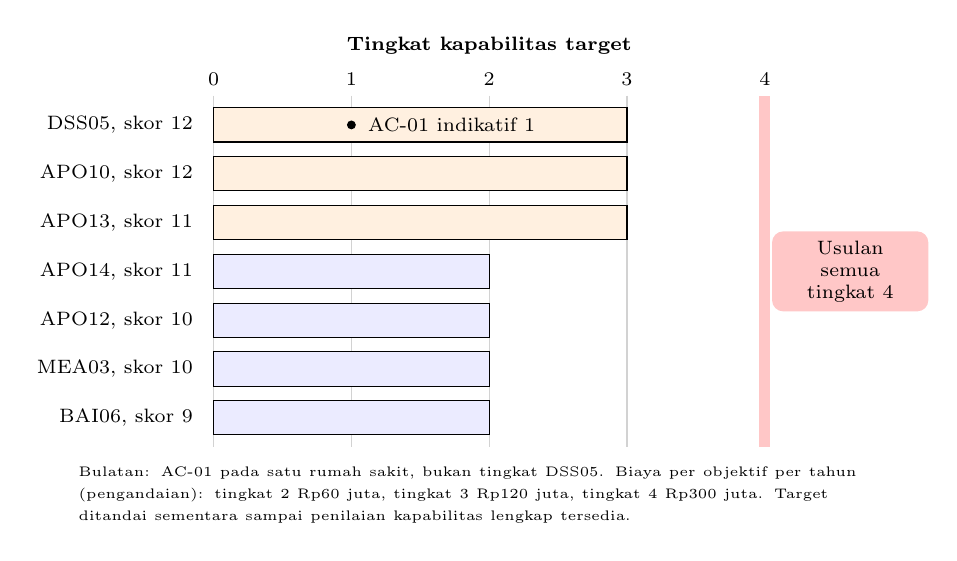
\begin{tikzpicture}[
  font=\scriptsize,
  x=1.75cm,
  y=0.62cm,
  batang3/.style={draw, fill=orange!12},
  batang2/.style={draw, fill=blue!8}]
  \foreach \tingkat in {0,1,2,3} {
    \draw[gray!35] (\tingkat,0.6) -- (\tingkat,-6.6);
    \node[above] at (\tingkat,0.6) {\tingkat};
  }
  \fill[red!22] (3.96,0.6) rectangle (4.04,-6.6);
  \node[above] at (4,0.6) {4};
  \node[fill=red!22, align=center, rounded corners, text width=1.75cm] at (4.62,-3)
    {Usulan\\semua\\tingkat 4};
  \node[above, font=\scriptsize\bfseries] at (2,1.25) {Tingkat kapabilitas target};
  \node[anchor=east] at (-0.08,0) {DSS05, skor 12};
  \node[anchor=east] at (-0.08,-1) {APO10, skor 12};
  \node[anchor=east] at (-0.08,-2) {APO13, skor 11};
  \node[anchor=east] at (-0.08,-3) {APO14, skor 11};
  \node[anchor=east] at (-0.08,-4) {APO12, skor 10};
  \node[anchor=east] at (-0.08,-5) {MEA03, skor 10};
  \node[anchor=east] at (-0.08,-6) {BAI06, skor 9};
  \draw[batang3] (0,-0.35) rectangle (3,0.35);
  \draw[batang3] (0,-1.35) rectangle (3,-0.65);
  \draw[batang3] (0,-2.35) rectangle (3,-1.65);
  \draw[batang2] (0,-3.35) rectangle (2,-2.65);
  \draw[batang2] (0,-4.35) rectangle (2,-3.65);
  \draw[batang2] (0,-5.35) rectangle (2,-4.65);
  \draw[batang2] (0,-6.35) rectangle (2,-5.65);
  \fill (1,0) circle (1.6pt);
  \node[anchor=west] at (1.05,0) {AC-01 indikatif 1};
  \node[anchor=north west, align=left, text width=10cm] at (-1.05,-6.8)
    {{\tiny\mdseries Bulatan: AC-01 pada satu rumah sakit, bukan tingkat DSS05. Biaya per objektif
    per tahun (pengandaian): tingkat 2 Rp60 juta, tingkat 3 Rp120 juta, tingkat 4 Rp300 juta.
    Target ditandai sementara sampai penilaian kapabilitas lengkap tersedia.}};
\end{tikzpicture}

  \caption{Target kapabilitas bertingkat dibanding usulan tingkat 4 (misalkan)}
  \label{fig:ch08-target-bertingkat}
\end{figure}

Dua objektif sengaja tidak mendapat target pada tabel itu. DSS04 menunggu analisis dampak bisnis
pada Bab 10, tetapi 144 uji pemulihan pada Paket B tetap berjalan. APO09 berskor 7 tetap
ditunda, walaupun praktik tingkat layanan tetap dipakai pada seksi ITIL. Penundaan target tidak
menghentikan pekerjaan yang sudah diwajibkan.

\begin{kasus}[title={Kasus Medikara Health: Usulan Tingkat 4 untuk Semua Objektif}]
Misalkan konsultan mengusulkan tingkat 4 untuk ketujuh objektif, dengan alasan angka terukur
mudah dilaporkan. Misalkan pula biaya per objektif per tahun Rp60 juta untuk tingkat 2, Rp120
juta untuk tingkat 3, dan Rp300 juta untuk tingkat 4. Pada DSS05, angka Rp120 juta sudah
mencakup AC-01 sebesar Rp60 juta. Usulan konsultan menelan 7 kali Rp300 juta, atau Rp2,1 miliar
per tahun. Rancangan bertingkat menelan 3 kali Rp120 juta ditambah 4 kali Rp60 juta, atau Rp600
juta. Selisihnya Rp1,5 miliar per tahun.

Keputusan ini punya tiga konsekuensi. Pertama, pada DSS05 saja, kenaikan dari tingkat 3 ke
tingkat 4 menambah Rp180 juta. Setelah AC-01, peluang R-01 menjadi 0,05 dengan kerugian
rata-rata Rp500 juta, sehingga harapan kerugiannya Rp25 juta per tahun. Sekalipun tingkat 4
menghapus seluruh sisa risiko itu, manfaatnya hanya Rp25 juta. Kedua, peluang kerugian Rp1,5
miliar atau lebih pada R-01 sudah 1 persen, di dalam batas 2 persen pada Bab 5. Ketiga, Rp600
juta melewati batas Rp400 juta, sehingga keputusan tetap naik ke direksi, bukan berhenti di
komite pengarah TI.

Hitungan rupiah bukan satu-satunya pertimbangan. Keselamatan pasien dan hak pasien tidak diukur
dengan harapan kerugian saja. Target ditinjau lagi bila AC-01 gagal pada tiga peninjauan
berturut-turut, bila ada kewajiban baru, atau bila arsitektur target berubah.

Rp600 juta adalah rancangan awal untuk tujuh objektif. Setelah analisis dampak bisnis selesai, Bab
10 menambahkan DSS04 pada tingkat 3 dengan kode T-24. Rancangannya menjadi 4 kali Rp120 juta
ditambah 4 kali Rp60 juta, atau Rp720 juta per tahun, dan keputusan tetap berada di direksi. Bab 14
memakai angka Rp720 juta.
\end{kasus}

Hitungan batas risiko dapat dipakai dengan arah sebaliknya. Misalkan kerugian Rp2 miliar pada
R-05 terjadi setiap kali pemulihan gagal. Dengan peluang 0,1, peluang kerugian Rp1,5 miliar atau
lebih adalah 10 persen, jauh di atas batas 2 persen. Peluangnya harus turun menjadi seperlima.
Karena itu, Paket B tidak dapat dipangkas walaupun skor R-05 lebih rendah daripada R-01.

\begin{pendalaman}
Souza Neto dan rekan mengusulkan penyempurnaan. Target ditetapkan satu tingkat demi satu tingkat,
dari tingkat 2 sampai tingkat 5. Tiap aktivitas diberi peringkat N, P, L, atau F, dengan
\textit{Not} di bawah 15 persen, \textit{Partially} 15 sampai 50 persen, \textit{Largely} 50
sampai 85 persen, dan \textit{Fully} lebih dari 85 persen. Proses naik hanya bila aktivitas pada
tingkat itu berperingkat L atau F. Mereka juga memetakan keluaran proses berskor rendah ke proses
berskor tinggi. MEA02 mendapat tingkat 2 pada contoh panduan, tetapi mengirim keluaran ke enam
objektif berskor tertinggi, sehingga tingkat rendah tidak patut diberikan otomatis
\cite{c04-kapabilitas}.

Metode ini usulan penulis, bukan aturan asesmen ISACA. Biaya penilaiannya dapat dihitung dari
asumsi Bab 4. Tujuh objektif dengan rata-rata 35 aktivitas berarti 245 aktivitas, atau 122,5 jam
pada 30 menit per aktivitas. Pada Medikara, BAI06 berskor paling rendah, tetapi Bab 4 menunjukkan
perubahan di rumah sakit Bogor ikut merusak data pada APO14. Keterkaitan seperti itu dapat
menjadi alasan menaikkan target BAI06 pada tahun kedua.
\end{pendalaman}

\section{Profil Target NIST CSF}

\subsection*{Profil target menyebut hasil yang dipilih}

Bab 6 menyerahkan profil target kepada bab ini. Profil target menyebut hasil yang dipilih dan
diprioritaskan organisasi untuk mencapai sasaran pengelolaan risiko keamanannya. Profil itu juga
memperhitungkan perubahan yang diperkirakan, seperti persyaratan baru, adopsi teknologi baru,
dan tren ancaman. Selisih dengan profil saat ini dianalisis, lalu menjadi rencana tindakan
berprioritas \cite{nistcsf2}. Bab 6 mengerjakan langkah 1 sampai 4 untuk profil
saat ini dengan pembanding sementara. Bab ini mengisi kolom target pada langkah 3, menyelesaikan
analisis celah pada langkah 4, dan menyiapkan langkah 5.

Analogi pemeriksaan kesehatan berkala membantu. Hasil laboratorium menunjukkan keadaan saat ini.
Dokter menetapkan sasaran berbeda untuk gula darah, kolesterol, dan tekanan darah sesuai risiko
pasien. Tidak semua angka harus sempurna pada bulan yang sama.

Dua contoh menuntut ukuran hasil yang nyata:
\begin{enumerate}
  \item Misalkan target PR.AA-05 mencakup 5 rumah sakit dalam 6 bulan. Penerimaan memerlukan 30
  dari 30 catatan peninjauan selama 6 bulan itu, atau 60 dari 60 per tahun. Pelatihan
  administrator saja tidak cukup.
  \item Misalkan pembukaan data asuransi untuk 72.000 klaim per tahun membutuhkan inventaris
  alur, penilaian dampak, serta batas akses. Forum arsitektur memeriksa kesesuaiannya dengan
  rancangan platform IT40613 dan layanan cloud IT40713. NIST juga menyebut profil target dapat
  menyatakan persyaratan kepada pemasok dan mitra \cite{nistcsf2}. Karena itu, laporan 12 jam
  dan 11 butir perjanjian dapat masuk kontrak vendor pada Bab 9.
\end{enumerate}

Tabel~\ref{tab:ch08-profil-target} menyusun profil target Medikara. Empat belas baris pertama
berasal dari profil saat ini Bab 6, dengan cakupan 5 rumah sakit dan Medikara+. Dua baris
terakhir, GV.PO-01 dan GV.PO-02, ditambahkan karena bab ini menata kebijakan. NIST merumuskan
keduanya sebagai kebijakan pengelolaan risiko keamanan yang ditetapkan, dikomunikasikan,
ditegakkan, dan ditinjau \cite{nistcsf2}. Keduanya belum pernah dinilai, sehingga profil menjadi
16 dari 106 subkategori dan kolom saat ini harus diisi lebih dahulu. Pada tabel, Multi-Factor
Authentication (MFA) mengikuti Bab 6, dan Gel. 2 berarti gelombang kedua.

\begin{table}[!htb]
  \centering\footnotesize
  \caption{Profil target NIST CSF Medikara untuk 12 bulan (misalkan)}
  \label{tab:ch08-profil-target}
  \begin{tabularx}{\textwidth}{|>{\raggedright\arraybackslash}p{0.13\textwidth}|>{\raggedright\arraybackslash}p{0.13\textwidth}|>{\raggedright\arraybackslash}p{0.11\textwidth}|>{\raggedright\arraybackslash}X|>{\raggedright\arraybackslash}p{0.07\textwidth}|}
    \hline
    \textbf{Subkategori} & \textbf{Saat ini} & \textbf{Target} & \textbf{Bukti penerimaan} &
    \textbf{Paket} \\ \hline
    GV.OC-03 & Sebagian & Terbukti & 16 dari 16 baris register terverifikasi & Umum \\ \hline
    GV.RM-02 & Sebagian & Terbukti & Batas diuji dengan satu penyimpangan & Umum \\ \hline
    GV.RR-02 & Sebagian & Terbukti & Mandat dan RACI disahkan; 120 akun berpemilik & A \\ \hline
    GV.SC-07 & Sebagian & Terbukti & Tinjauan vendor berkala; 11 dari 11 butir & A, C \\ \hline
    ID.AM-02 & Sebagian & Sebagian & Rekonsiliasi berjalan pada 2 dari 5 rumah sakit & Gel. 2 \\
    \hline
    PR.AA-01 & Sebagian & Sebagian & Nol akun bersama pada sampel 2 rumah sakit & Gel. 2 \\
    \hline
    PR.AA-03 & Sebagian & Terbukti & MFA pada 120 dari 120 akun & A \\ \hline
    PR.AA-05 & Sebagian & Terbukti & 120 dari 120 akun cocok; 60 dari 60 catatan & A \\ \hline
    PR.AA-06 & Tidak relevan & Tidak relevan & Ditinjau bila vendor hadir di lokasi & Umum \\
    \hline
    PR.PS-04 & Terbukti & Terbukti & Cakupan ditambah Medikara+; catatan rinci 90 hari & D \\
    \hline
    PR.DS-11 & Sebagian & Terbukti & Cadangan disertai hasil uji pemulihan & B \\ \hline
    DE.CM-03 & Sebagian & Terbukti & 247 dari 260 tinjauan mingguan & D \\ \hline
    RS.MA-01 & Belum ada bukti & Terbukti & 2 latihan bersama; laporan vendor dalam 12 jam & C \\
    \hline
    RC.RP-03 & Belum ada bukti & Terbukti & 144 uji per tahun; hasil disahkan & B \\ \hline
    GV.PO-01 & Belum dinilai & Terbukti & KB-01 dan KB-05 disahkan serta disosialisasikan & Umum
    \\ \hline
    GV.PO-02 & Belum dinilai & Terbukti & 8 dari 8 dokumen ditinjau sesuai jadwal & Umum \\
    \hline
  \end{tabularx}
\end{table}

Pembacaan tabel memberi dua hal. Pada 14 baris Bab 6, status terbukti naik dari 1 menjadi 11,
sebagian turun dari 10 menjadi 2, dan belum ada bukti turun dari 2 menjadi 0. Satu baris tetap
tidak relevan. Selain itu, ID.AM-02 dan PR.AA-01 sengaja tetap sebagian, karena G-06 dan G-04
masuk gelombang kedua. Profil target yang semua barisnya terbukti pada tahun pertama sering
menandakan pilihan belum dibuat.

Perubahan yang diperkirakan juga masuk rancangan. Bab 7 mencatat Peraturan Pemerintah (PP)
33/2026 berlaku 16 Januari 2027, tetapi naskah resminya belum diperoleh, sehingga aturan itu
tetap menjadi butir pemantauan \cite{bpom-pp33-2026-status}. Rencana modernisasi ke cloud pada
IT40713 dapat mengubah cakupan PR.DS-11 dan RC.RP-03. Bila arsitektur berubah, baris yang
terkena ditinjau ulang.

\subsection*{Tier tidak dihitung dari profil}

Dua hal pada profil target sering tertukar: target hasil dan \textit{tier}. Pembagiannya begini.
Target hasil menyebut apa yang harus tercapai. \textit{Tier} menggambarkan ketelitian pengelolaan
risiko. NIST mendorong kenaikan \textit{tier} bila risiko atau mandat lebih besar, atau bila
analisis biaya dan manfaat menunjukkan penurunan risiko yang layak \cite{nistcsf2}.

Tabel~\ref{tab:ch08-tiga-target} melanjutkan batas pada Bab 6. Ketiga ukuran tidak saling
dikonversi. Medikara menuju Tier 3 untuk Protect karena R-01 dan K-01 merupakan risiko dan mandat
yang besar. Pada Bab 6, Tier 3 berarti praktik disetujui resmi sebagai kebijakan dan diperbarui
berkala, sehingga arsitektur kebijakan pada bab ini menjadi syaratnya. Tier 4 memerlukan
informasi pemasok yang hampir waktu nyata. Medikara belum menjadikannya target, karena biayanya
belum dapat dibenarkan pada tahun pertama.

\begin{table}[!htb]
  \centering\small
  \caption{Tiga target yang tidak saling dikonversi (misalkan)}\label{tab:ch08-tiga-target}
  \begin{tabularx}{\textwidth}{|>{\raggedright\arraybackslash}p{0.22\textwidth}|>{\raggedright\arraybackslash}X|>{\raggedright\arraybackslash}X|}
    \hline
    \textbf{Ukuran} & \textbf{Saat ini} & \textbf{Target} \\ \hline
    Status lokal PR.AA-05 & Sebagian, bukti 1 dari 5 rumah sakit & Terbukti pada 5 rumah sakit \\
    \hline
    \textit{Tier} Protect & Tier 2 pada pembacaan pimpinan & Tier 3 pada pembacaan pimpinan \\
    \hline
    Tingkat kapabilitas DSS05 & Indikatif 1 lewat AC-01 pada satu rumah sakit & Tingkat 3 setelah
    penilaian lengkap \\ \hline
  \end{tabularx}
\end{table}

\section{Struktur, Forum Keputusan, dan Pemisahan Tugas}

\subsection*{Forum dan peran kunci}

Hasil target menentukan kewenangan yang diperlukan. Struktur tata kelola membagi hak keputusan
dan pengawasan. Forum harus memiliki mandat, anggota, kuorum, jenis keputusan, jalur eskalasi,
serta catatan hasil. ISO/IEC 38500:2024 memakai tugas evaluasi, pengarahan, dan pemantauan, lalu
menambahkan pelibatan pemangku kepentingan \cite{c02-iso-perubahan}. Peterson memandang struktur,
proses, dan hubungan kerja sebagai satu kesatuan \cite{c02-peterson2004}. Forum tanpa proses
hanya menambah rapat.

Beberapa peran kunci perlu dibedakan. Chief Information Security Officer (CISO), yang pada mata
kuliah lain disebut kepala keamanan informasi, mengoordinasikan keamanan. Petugas pelindungan data memberi penilaian sesuai tugas dan independensinya. Pemilik
data menetapkan aturan pemakaian data. Pemilik layanan bertanggung jawab atas hasil layanan.
Forum arsitektur (\textit{architecture board}) memeriksa kesesuaian rancangan dengan prinsip
arsitektur. Rincian forum arsitektur dibahas pada mata kuliah IT40513.

Analogi rapat pengelola gedung menunjukkan perlunya mandat. Petugas perawatan dapat memperbaiki
lampu. Ia tidak otomatis berwenang mengubah jalur evakuasi atau menerima risiko keselamatan
penghuni.

Dua contoh menghindari persetujuan yang berputar:
\begin{enumerate}
  \item Misalkan usulan data asuransi berjalan berurutan melewati 4 forum bulanan. Waktu
  tunggunya paling lama 4 bulan. Dengan 5 menit per klaim, 6.000 klaim manual memakan 500 jam per
  bulan, atau Rp30 juta per bulan. Empat bulan berarti Rp120 juta. Alur pada
  Gambar~\ref{fig:ch08-alur-data} selesai dalam 10 hari kerja, sekitar setengah bulan atau Rp15
  juta. Selisihnya Rp105 juta, dan tinjauan hukum, privasi, keamanan, serta arsitektur tetap ada.
  \item Misalkan Medikara mencatat 40 perubahan per bulan: 30 kecil, 8 biasa, dan 2 darurat. Bila
  semuanya dibawa ke komite pengarah TI selama 5 menit per usulan, diperlukan 200 menit. Bab 2
  menyediakan rapat 120 menit per bulan. Perubahan kecil tampilan janji temu yang tidak mengubah
  data atau kendali keamanan memakai persetujuan terdelegasi bila kriteria dan bukti pengujiannya
  terpenuhi.
\end{enumerate}

Tabel~\ref{tab:ch08-forum} merangkum rancangan forum dan peran. Komite pengarah TI dan batas
delegasi mengikuti Bab 2. Keanggotaan komite risiko dan forum arsitektur merupakan pengandaian
bab ini. Komite risiko beranggotakan direktur keuangan sebagai ketua, direktur pelayanan, kepala
risiko, hukum, dan CISO. Pada tabel, Data Protection Impact Assessment (DPIA) mengikuti Bab 7.
Gambar~\ref{fig:ch08-peta-peran} menempatkan semuanya pada Three Lines Model dari Bab 1.

\begin{table}[!htb]
  \centering\small
  \caption{Rancangan forum dan peran Medikara (misalkan)}\label{tab:ch08-forum}
  \begin{tabularx}{\textwidth}{|>{\raggedright\arraybackslash}p{0.2\textwidth}|>{\raggedright\arraybackslash}X|>{\raggedright\arraybackslash}X|>{\raggedright\arraybackslash}p{0.2\textwidth}|}
    \hline
    \textbf{Forum atau peran} & \textbf{Mandat} & \textbf{Aturan kerja} & \textbf{Bukti hasil} \\
    \hline
    Direksi & Risiko di atas batas; keputusan di atas Rp400 juta sampai Rp5 miliar & Laporan
    triwulan ke dewan komisaris & Keputusan, alasan, batas waktu \\ \hline
    Komite pengarah TI & Prioritas dan anggaran lintas fasilitas sampai Rp400 juta & 9 anggota,
    kuorum 6; bulanan 2 jam & Notulen dan pemilik manfaat \\ \hline
    Komite risiko & Menelaah risiko di atas batas; memberi rekomendasi ke direksi & 5 anggota,
    kuorum 4; triwulanan 2 jam & Rekomendasi dan pemantauan batas \\ \hline
    Forum arsitektur & Kesesuaian rancangan dan pengecualian standar & 6 anggota; dua kali sebulan
    1 jam; kepala TI memutuskan & Catatan keputusan arsitektur \\ \hline
    Direktur pelayanan & Akuntabilitas rekam medis terpadu dan tujuan berbagi data & Naik ke
    direksi bila melewati batas & Keputusan tujuan dan mutu layanan \\ \hline
    Kepala rekam medis & Pemilik data; aturan data rekam medis & Hak henti bila dasar pemrosesan
    belum ada & Catatan henti dan alasan \\ \hline
    Pemilik layanan & Hasil layanan, akses teknis, uji pemulihan & Pengecualian darurat paling
    lama 24 jam & Catatan AC-01, hasil uji \\ \hline
    CISO & Koordinasi keamanan dan tinjauan standar & Lini kedua; tidak menyetujui akses & Pendapat
    dan temuan tertulis \\ \hline
    Petugas pelindungan data & Pendapat DPIA dan pemantauan pemrosesan & 1 penuh waktu, 5
    koordinator 20 persen & Pendapat DPIA \\ \hline
  \end{tabularx}
\end{table}

\begin{figure}[!htb]
  \centering
  \begin{tikzpicture}[
  font=\scriptsize,
  kotak/.style={draw, rounded corners, align=center, text width=3cm, minimum height=1.1cm},
  panah/.style={-{Stealth[length=2mm]}, thick}]
  \node[draw, rounded corners, align=center, text width=10.5cm, minimum height=0.9cm,
    fill=praditagreen!15] (bp) at (0,0)
    {\textbf{Badan pengarah}\\Dewan komisaris mengawasi; direksi memutuskan sesuai kewenangan};
  \node[kotak, fill=blue!8] (fa) at (-3.75,-1.75)
    {\textbf{Forum arsitektur}\\standar dan pola integrasi};
  \node[kotak, fill=blue!8] (kp) at (0,-1.75)
    {\textbf{Komite pengarah TI}\\9 anggota, sampai Rp400 juta};
  \node[kotak, fill=blue!8] (kr) at (3.75,-1.75)
    {\textbf{Komite risiko}\\5 anggota, rekomendasi risiko};
  \node[kotak, fill=orange!12, minimum height=1.5cm] (l1) at (-3.75,-3.85)
    {\textbf{Lini pertama}\\direktur pelayanan, pemilik layanan, kepala rekam medis, operasi TI};
  \node[kotak, fill=blue!8, minimum height=1.5cm] (l2) at (0,-3.85)
    {\textbf{Lini kedua}\\CISO, petugas pelindungan data, kepala risiko, hukum};
  \node[kotak, fill=green!10, minimum height=1.5cm] (l3) at (3.75,-3.85)
    {\textbf{Lini ketiga}\\audit internal, asurans independen};
  \draw[panah] (fa) -- (kp);
  \draw[panah] (kp) -- (kp |- bp.south);
  \draw[panah] (kr) -- (kr |- bp.south);
  \draw[panah] (l1) -- (fa);
  \draw[panah] (l1.north east) -- (kp.south west);
  \draw[panah] (l2.north east) -- (kr.south west);
  \draw[panah] (l2.south) -- ++(0,-0.3) -| (l1.south)
    node[pos=0.25, below] {{\tiny\mdseries memantau dan menantang}};
  \draw[panah] (l3.east) -- ++(0.28,0) |- (bp.east);
\end{tikzpicture}

  \caption{Forum dan peran pada Three Lines Model (misalkan)}
  \label{fig:ch08-peta-peran}
\end{figure}

Penunjukan petugas pelindungan data menutup CP-06. Bab 7 mengandaikan kapasitasnya setara 2 orang
penuh waktu, dan kepala TI tidak merangkap peran itu. CISO berada pada lini kedua. Three Lines
Model membedakan peran, bukan departemen \cite{iia-tlm2026}, sehingga bila fungsi keamanan juga
menjalankan tinjauan catatan aktivitas pada G-02, peran pelaksana dan peran penantang perlu
dipegang orang berbeda.

Pertanyaan berikutnya: apakah Medikara perlu komite risiko terpisah? Biaya forum dapat dihitung.
Komite pengarah TI memakan $9 \times 2 \times 12 = 216$ jam orang per tahun. Komite risiko
memakan $5 \times 2 \times 4 = 40$ jam. Forum arsitektur memakan $6 \times 1 \times 24 = 144$ jam.
Jumlahnya 400 jam, atau sekitar Rp24 juta pada tarif Rp60.000 per jam. Biaya sesungguhnya lebih
tinggi karena tarif pimpinan lebih mahal. Pilihan lain adalah agenda risiko triwulanan pada
komite pengarah TI, yang menghemat 40 jam tetapi menambah agenda pada rapat 2 jam yang sudah
padat. Misalkan Medikara memilih komite terpisah karena R-11 dan K-04 memerlukan pembahasan yang
tidak bercampur dengan anggaran. Organisasi kecil dapat memilih sebaliknya. Yang dinilai adalah
kemampuan forum mengambil keputusan, bukan banyaknya forum.

\begin{kasus}[title={Kasus Medikara Health: Dua Pertanyaan C3}]
Pertanyaan pertama: siapa menyetujui pembukaan data kepada mitra? Misalkan direktur pelayanan
memutuskan tujuan berbagi data. Pemilik layanan mengusulkan tujuan dan data minimum. Petugas
pelindungan data menyusun pendapat atas DPIA, yang pada Bab 7 memerlukan 72 jam dalam 3 hari
kerja. Hukum, keamanan, dan forum arsitektur meninjau secara paralel selama 5 hari kerja. Kepala
rekam medis memegang hak henti sempit bila dasar pemrosesan belum ada. Risiko sisa di atas batas
naik ke direksi. Gambar~\ref{fig:ch08-alur-data} merangkum alurnya.

Pertanyaan kedua: siapa memegang akuntabilitas atas rekam medis terpadu? Misalkan direktur
pelayanan memegangnya. Peran itu sejalan dengan Bab 2, yang menempatkannya sebagai pemilik manfaat
layanan, dan Bab 5, yang menempatkannya sebagai pemilik R-11. Kepala rekam medis menjalankan aturan
data. Kepala TI menjalankan platform, tetapi tidak memegang akuntabilitas hasil klinis.

Rancangan ini punya tiga konsekuensi. Pertama, jalur tinjauan menjadi lebih pendek. Tinjauan
berurutan oleh hukum, keamanan, dan arsitektur memakan 15 hari kerja, sehingga seluruh alur
menjadi 20 hari kerja. Tinjauan paralel membuatnya 10 hari kerja. Kedua, peluang lolos naik. Bab 2
menghitung empat veto dengan persetujuan 90 persen menghasilkan 65,6 persen. Dengan satu hak henti
sempit, angka itu menjadi 90 persen, dan masukan pihak lain wajib didengar serta dijawab tertulis.
Ketiga, mandat internal tidak menghapus aturan. Bab 3 mencatat Permenkes 24/2022 Pasal 30: hak
akses ditetapkan pimpinan fasilitas \cite{permenkes24-2022}. Model menyediakan aturan yang sama,
tetapi penetapan pada 36 fasilitas tetap harus ada. Tafsir hukum atas susunan ini perlu
dikonfirmasi kepada fungsi hukum.
\end{kasus}

\begin{figure}[!htb]
  \centering
  \begin{tikzpicture}[
  font=\scriptsize,
  tahap/.style={draw, rounded corners, align=center, text width=2.4cm,
    minimum height=1.3cm, fill=blue!8},
  panah/.style={-{Stealth[length=2mm]}, thick}]
  \node[tahap] (n1) at (0,0)
    {Usulan tujuan dan data minimum\\{\tiny\mdseries pemilik layanan, hari 1}};
  \node[tahap] (n2) at (3,0)
    {DPIA\\{\tiny\mdseries petugas pelindungan data, hari 2 sampai 4}};
  \node[tahap] (n3) at (6,0)
    {Tinjauan paralel\\{\tiny\mdseries hukum, keamanan, arsitektur, hari 5 sampai 9}};
  \node[tahap, fill=orange!12] (n4) at (9,0)
    {Keputusan tujuan\\{\tiny\mdseries direktur pelayanan, hari 10}};
  \node[tahap, fill=red!22] (h1) at (3,-2.1)
    {Dasar pemrosesan belum ada\\{\tiny\mdseries kepala rekam medis menghentikan}};
  \node[tahap, fill=gray!35] (h2) at (6,-2.1)
    {Risiko sisa di atas batas\\{\tiny\mdseries naik ke direksi}};
  \node[tahap, fill=green!10] (h3) at (9,-2.1)
    {Akses teknis mitra\\{\tiny\mdseries pemilik layanan, operasi TI}};
  \draw[panah] (n1) -- (n2);
  \draw[panah] (n2) -- (n3);
  \draw[panah] (n3) -- (n4);
  \draw[panah] (n2) -- (h1);
  \draw[panah] (n4) -- (h2);
  \draw[panah] (n4) -- (h3);
\end{tikzpicture}

  \caption{Alur persetujuan pembukaan data kepada mitra dalam 10 hari kerja (misalkan)}
  \label{fig:ch08-alur-data}
\end{figure}

\subsection*{Pemisahan tugas}

Pemisahan tugas membatasi pihak yang mengusulkan, menyetujui, menjalankan, dan menguji. NIST
menyebut pemisahan tugas sebagai salah satu kontrol akses \cite{c08-nist-sp80012r1}. Tujuannya
sederhana: tidak ada satu orang yang dapat membuat masalah sekaligus menutupinya.

Analogi kas kecil kantor menjelaskan alasannya. Orang yang mengeluarkan uang tidak mencocokkan
buku kasnya sendiri. Pencocokan oleh orang lain membuat selisih lebih cepat terlihat.

Dua contoh memperlihatkan penerapannya:
\begin{enumerate}
  \item Tabel~\ref{tab:ch08-pemisahan} menerapkan empat tugas pada AC-01. Administrator tidak
  menyetujui aksesnya sendiri. Audit internal menguji secara independen, dan contoh pada Bab 6
  memakai 30 akun sampel, dengan 24 akun sesuai.
  \item Misalkan satu klinik hanya memiliki 1 administrator. Pemisahan penuh tidak mungkin,
  sehingga Medikara memakai pemeriksaan kompensasi oleh peninjau pusat. Pada 18 klinik, peninjauan
  bulanan 15 menit per klinik memakan 54 jam per tahun. Potensi konflik dan bukti tinjauannya
  tetap dicatat.
\end{enumerate}

\begin{table}[!htb]
  \centering\small
  \caption{Pemisahan tugas pada AC-01 (misalkan)}\label{tab:ch08-pemisahan}
  \begin{tabularx}{\textwidth}{|>{\raggedright\arraybackslash}p{0.18\textwidth}|>{\raggedright\arraybackslash}p{0.27\textwidth}|>{\raggedright\arraybackslash}X|}
    \hline
    \textbf{Tugas} & \textbf{Pemegang} & \textbf{Bukti} \\ \hline
    Mengusulkan & Pengelola vendor & Daftar penugasan dan tanggal berakhir \\ \hline
    Menyetujui & Pemilik Medikara+ & Persetujuan per akun \\ \hline
    Menjalankan & Operasi TI & Tiket pemberian dan pencabutan \\ \hline
    Menguji & Audit internal & Hasil uji sampel dan temuan \\ \hline
  \end{tabularx}
\end{table}

\section{Matriks RACI yang Dapat Dipakai}

RACI membedakan pelaksana, pemegang akuntabilitas, pihak yang dimintai pertimbangan, dan pihak
yang diberi informasi. Dalam rancangan kelas ini setiap baris memiliki satu \textit{Accountable}
agar keputusan akhir jelas. Satu orang boleh menjalankan beberapa peran bila kewenangan dan
pemisahan tugas tetap dapat dipertanggungjawabkan.

Analogi pengelolaan acara memperjelas pembagian. Banyak panitia menjalankan kegiatan, tetapi satu
penanggung jawab menetapkan keputusan akhir untuk satu kegiatan. Bila dua pihak sama-sama
menganggap yang lain memutuskan, pekerjaan berhenti.

Dua contoh menunjukkan perlunya unit keputusan yang tepat:
\begin{enumerate}
  \item Misalkan baris berjudul ``mengelola seluruh data'' diberi dua \textit{Accountable}, yaitu
  TI dan pimpinan klinis. Tim memecahnya menjadi aturan rekam medis, tujuan berbagi data, akses
  teknis, dan uji pemulihan. Satu baris kabur menjadi 4 baris dengan pemegang akuntabilitas yang
  jelas.
  \item Bab 2 menempatkan pemberian akses vendor pada D-06, dengan pemilik Medikara+ sebagai
  pemutus dan eskalasi ke direktur pelayanan bila kepala TI keberatan. Model target menulisnya
  sebagai satu \textit{Accountable}, yaitu pemilik layanan, dan operasi TI sebagai
  \textit{Responsible}. Keamanan memberi pertimbangan. Administrator tidak menyetujui aksesnya
  sendiri.
\end{enumerate}

Dua hal sering tertukar: \textit{Accountable} dan \textit{Responsible}. Pembagiannya begini.
\textit{Responsible} mengerjakan. \textit{Accountable} menanggung keputusan akhir dan menjawab
bila hasilnya gagal. Kepala operasi TI dapat menjalankan 144 uji pemulihan, sedangkan pemilik
layanan yang mengesahkan apakah layanannya benar-benar pulih.

Tabel~\ref{tab:ch08-raci} merangkum 10 keputusan dengan 9 peran. Salinannya tersedia di
\berkas{sources/chapter08/contoh-raci-medikara.csv}. Audit internal sengaja tidak masuk matriks,
karena peran lini ketiga menguji hasil kerja dan tidak ikut memutuskan.

\begin{table}[!htb]
  \centering\small
  \caption{Contoh RACI keputusan target Medikara (misalkan)}\label{tab:ch08-raci}
  \begin{tabularx}{\textwidth}{|>{\raggedright\arraybackslash}X|*{9}{>{\centering\arraybackslash}p{0.042\textwidth}|}}
    \hline
    \textbf{Keputusan} & \textbf{Dir} & \textbf{DP} & \textbf{PL} & \textbf{RM} & \textbf{TI} &
    \textbf{KA} & \textbf{PD} & \textbf{HK} & \textbf{FA} \\ \hline
    1. Aturan rekam medis terpadu & I & A & C & R & C & C & C & C & C \\ \hline
    2. Tujuan berbagi data mitra & I & A & R & C & I & C & C & C & C \\ \hline
    3. Akses teknis mitra & - & I & A & C & R & C & I & I & C \\ \hline
    4. Peninjauan akses AC-01 & I & I & A & - & R & C & I & - & - \\ \hline
    5. Pencabutan akun vendor & - & - & A & - & R & C & I & - & - \\ \hline
    6. Perubahan darurat SIMRS & I & C & A & C & R & C & I & - & I \\ \hline
    7. Penerimaan risiko di atas batas & A & C & R & C & C & C & C & C & I \\ \hline
    8. Uji pemulihan & I & I & A & C & R & C & - & - & I \\ \hline
    9. Pemberitahuan insiden data & I & C & C & C & C & R & R & A & - \\ \hline
    10. Subprosesor dan penghentian vendor & I & C & A & C & R & C & C & C & C \\ \hline
  \end{tabularx}

  \vspace{4pt}
  {\footnotesize Dir direksi; DP direktur pelayanan; PL pemilik layanan; RM kepala rekam medis;
  TI operasi TI; KA keamanan (CISO); PD petugas pelindungan data; HK hukum; FA forum arsitektur.}
\end{table}

Matriks itu dapat dibaca seperti data. Huruf A berjumlah 10, dan tiap baris mempunyai tepat satu
A. Pemilik layanan memegang 6 dari 10 A. Angka itu aman hanya bila peran tersebut dipegang
beberapa orang, misalnya pemilik Medikara+ dan pemilik SIMRS, dengan pengganti yang ditunjuk.
Keamanan muncul sebagai C pada 9 dari 10 baris. Misalkan tiap baris terjadi 4 kali per bulan dan
satu pertimbangan memerlukan 2 jam. Bebannya $9 \times 4 \times 2 = 72$ jam per bulan, atau 45
persen dari 160 jam kerja. Kolom C terbanyak menjadi antrean. Bila baris 4 dan 5 memakai kriteria
tetap sehingga keamanan cukup menjadi I, bebannya turun menjadi 56 jam, atau 35 persen.

RACI tidak menggantikan wewenang dalam piagam atau aturan hukum. Kolom C juga bukan hak veto
universal. Jika dua fungsi mempunyai persetujuan terpisah yang wajib, tim membuat baris keputusan
masing-masing dan menjelaskan ketergantungannya. Baris 2 dan baris 3 pada tabel adalah contohnya:
tujuan disetujui lebih dahulu, baru akses teknis diberikan.

Tiga bacaan memberi gambaran pemakaiannya. Feltus dan rekan mengajukan model tanggung jawab
karyawan yang dibangun atas kewajiban, hak, dan komitmen, membandingkannya dengan konsep pada COBIT,
lalu mengilustrasikan usulan perubahannya pada bagan RACI \cite{c08-feltus2009}. Michałek
merancang matriks RACI untuk organisasi proyek matriks dengan pendekatan \textit{design science research}, menerapkannya pada
tiga portofolio proyek pada 2023, lalu memvalidasi serta menyempurnakannya pada 2024
\cite{c08-michalek2026}. Hartono dan rekan memakai RACI untuk membagi kegiatan mitigasi setelah
analisis risiko pada satu usaha \cite{c08-hartono2024}. Abstrak ketiga sumber itu tidak
melaporkan angka hasil. Karena itu, bab ini memperlakukan aturan satu \textit{Accountable} sebagai
aturan rancangan yang perlu diuji lewat simulasi, bukan temuan yang berlaku umum.

\section{Arsitektur dan Siklus Hidup Kebijakan}

\subsection*{Empat jenis dokumen}

Kebijakan menyatakan arah dan tanggung jawab pada tingkat yang luas. NIST menjelaskan bahwa
organisasi karena itu menyusun standar, pedoman, dan prosedur agar pelaksanaannya lebih jelas.
Standar biasanya wajib di dalam organisasi. Pedoman membantu pelaksana dan dapat dijalankan dengan
lebih dari satu cara. Prosedur merinci langkah untuk menjalankan kebijakan, standar, dan pedoman
\cite{c08-nist-sp80012r1}. Setiap dokumen memiliki pemilik, versi, persetujuan, tanggal berlaku,
pelatihan, dan jadwal tinjau.

Analogi aturan perpustakaan memisahkan tingkatnya. Kebijakan menetapkan pelindungan koleksi.
Standar menetapkan lama peminjaman. Pedoman membantu petugas menghadapi kasus khusus. Prosedur
menjelaskan pencatatan dan pengembalian.

Dua contoh menunjukkan akibat dokumen yang tidak terhubung:
\begin{enumerate}
  \item Misalkan kebijakan mewajibkan akses sesuai tugas, tetapi prosedur keluar vendor tidak
  meminta pencabutan akun. Bab 6 menghitung pencabutan turun dari 24 menjadi 9, 5, dan 2 akun
  setelah prosedur itu diubah. Kalimat kebijakan tidak berubah sama sekali. Yang berubah adalah
  tautannya dengan langkah kerja.
  \item Misalkan standar masa simpan catatan rinci diusulkan menjadi 180 hari. Bab 7 sudah
  menghitung kenaikan dari 7 menjadi 90 hari menaikkan ruang simpan 12,9 kali. Angka 180 hari
  menaikkannya 25,7 kali dari 7 hari, dan menggandakan paparan data pribadi dibanding 90 hari. Tim
  menilai dasar serta tujuan sebelum menyetujui angka. Retensi rekam medis 25 tahun pada K-03
  tidak disalin ke semua jenis catatan.
\end{enumerate}

Gambar~\ref{fig:ch08-hierarki} memperlihatkan hubungannya. Standar dan pedoman ditempatkan sejajar,
karena keduanya menurunkan kebijakan dengan sifat yang berbeda. Tabel~\ref{tab:ch08-kebijakan}
menerapkan keempatnya pada akses vendor. NIST juga menyarankan pemisahan yang jelas antara
kebijakan dan pelaksanaannya, karena pemisahan itu memberi keleluasaan cara pelaksanaan
\cite{c08-nist-sp80012r1}.

\begin{figure}[!htb]
  \centering
  \begin{tikzpicture}[
  font=\scriptsize,
  lapis/.style={draw, rounded corners, align=center, minimum height=0.95cm},
  catatan/.style={anchor=west, align=left, text width=4.5cm},
  panah/.style={-{Stealth[length=2mm]}, thick}]
  \node[lapis, fill=praditagreen!15, text width=5.8cm] (kb) at (0,0)
    {\textbf{Kebijakan}\\arah dan tanggung jawab};
  \node[lapis, fill=blue!8, text width=2.7cm] (st) at (-1.55,-1.45)
    {\textbf{Standar}\\ketentuan wajib};
  \node[lapis, fill=blue!8, text width=2.7cm] (pd) at (1.55,-1.45)
    {\textbf{Pedoman}\\pilihan pelaksanaan};
  \node[lapis, fill=orange!12, text width=5.8cm] (pr) at (0,-2.9)
    {\textbf{Prosedur}\\langkah kerja yang dapat diuji};
  \node[lapis, fill=green!10, text width=5.8cm] (bk) at (0,-4.35)
    {\textbf{Bukti operasi}\\catatan AC-01, tiket pencabutan, hasil uji};
  \draw[panah] (kb.south -| st) -- (st);
  \draw[panah] (kb.south -| pd) -- (pd);
  \draw[panah] (st) -- (pr.north -| st);
  \draw[panah] (pd) -- (pr.north -| pd);
  \draw[panah] (pr) -- (bk);
  \node[catatan] at (3.35,0) {KB-01, KB-05\\Disetujui direksi; tinjau 24 bulan};
  \node[catatan] at (3.35,-1.45)
    {KB-02, KB-06 disetujui komite pengarah TI; KB-04 disetujui direktur pelayanan; tinjau
    12 bulan};
  \node[catatan] at (3.35,-2.9)
    {KB-03, KB-07, KB-08\\Disetujui kepala TI atau komite; tinjau 12 bulan};
  \node[catatan] at (3.35,-4.35) {Diperiksa terhadap bukti penerimaan};
\end{tikzpicture}

  \caption{Arsitektur kebijakan dan penyetujunya (misalkan)}
  \label{fig:ch08-hierarki}
\end{figure}

\begin{table}[!htb]
  \centering\small
  \caption{Hubungan jenis dokumen dan bukti pada akses vendor (misalkan)}
  \label{tab:ch08-kebijakan}
  \begin{tabularx}{\textwidth}{|>{\raggedright\arraybackslash}p{0.14\textwidth}|>{\raggedright\arraybackslash}X|>{\raggedright\arraybackslash}X|}
    \hline
    \textbf{Jenis} & \textbf{Isi akses vendor} & \textbf{Bukti} \\ \hline
    Kebijakan & Akses sesuai kebutuhan dan dapat ditelusuri & Persetujuan serta pemilik \\ \hline
    Standar & Akun pribadi, MFA, dan masa berlaku wajib & Daftar syarat pemeriksaan \\ \hline
    Pedoman & Contoh akses darurat terbatas & Contoh skenario dan pelatihan \\ \hline
    Prosedur & Beri, tinjau, dan cabut akun paling lambat 1 hari kerja & Catatan AC-01 dan tiket
    pencabutan \\ \hline
  \end{tabularx}
\end{table}

\subsection*{Daftar kebijakan dan bebannya}

Pertanyaan kemudian muncul: dokumen mana yang benar-benar perlu ditulis? Medikara tidak mulai dari
daftar dokumen ideal. Medikara mulai dari celah. Tabel~\ref{tab:ch08-daftar-kebijakan} menurunkan
delapan dokumen dari paket target. Kodenya KB, karena awalan K sudah dipakai register kewajiban
Bab 3.

\begin{table}[!htb]
  \centering\footnotesize
  \caption{Daftar kebijakan yang dibuat atau direvisi (misalkan)}
  \label{tab:ch08-daftar-kebijakan}
  \begin{tabularx}{\textwidth}{|>{\raggedright\arraybackslash}p{0.08\textwidth}|>{\raggedright\arraybackslash}p{0.11\textwidth}|>{\raggedright\arraybackslash}X|>{\raggedright\arraybackslash}p{0.11\textwidth}|>{\raggedright\arraybackslash}p{0.17\textwidth}|>{\raggedright\arraybackslash}p{0.17\textwidth}|}
    \hline
    \textbf{ID} & \textbf{Jenis} & \textbf{Nama} & \textbf{Celah} & \textbf{Pemilik} &
    \textbf{Penyetuju} \\ \hline
    KB-01 & Kebijakan & Akses dan penggunaan data & G-01, G-04 & Kepala rekam medis & Direksi \\
    \hline
    KB-02 & Standar & Akun vendor & G-01, CP-01 & CISO & Komite pengarah TI \\ \hline
    KB-03 & Prosedur & AC-01 dan pencabutan & G-01 & Pemilik layanan & Kepala TI \\ \hline
    KB-04 & Pedoman & Akses darurat klinis & R-05, R-11 & Pimpinan klinis & Direktur pelayanan \\
    \hline
    KB-05 & Kebijakan & Berbagi data dengan mitra & CP-03 & Direktur pelayanan & Direksi \\ \hline
    KB-06 & Standar & Masa simpan catatan aktivitas & CP-05, G-02 & CISO & Komite pengarah TI \\
    \hline
    KB-07 & Prosedur & Pemberitahuan insiden & CP-04, G-05 & Fungsi hukum & Komite pengarah TI \\
    \hline
    KB-08 & Prosedur & Uji pemulihan & G-03 & Pemilik layanan & Kepala TI \\ \hline
  \end{tabularx}
\end{table}

Keputusan ini punya dua konsekuensi. Pertama, bebannya terukur. Misalkan kebijakan ditinjau tiap
24 bulan dan dokumen lain tiap 12 bulan, sehingga ada 7 tinjauan per tahun. Dengan 8 jam per
tinjauan, bebannya 56 jam. Pelatihan 2 jam untuk 52 staf TI menambah 104 jam. Jumlahnya 160 jam,
atau satu bulan kerja, senilai Rp9,6 juta. Kedua, perubahan menjadi lebih ringan. Direksi hanya
menyetujui 2 dari 8 dokumen. Enam dokumen lain dapat berubah tanpa rapat direksi, selama arahnya
tetap sama.

\subsection*{Pengecualian}

Pengecualian harus menyebut ruang lingkup, risiko sisa, kontrol kompensasi, pemberi persetujuan,
dan kedaluwarsa. Tanpa masa berlaku, pengecualian sementara dapat menjadi kebijakan tanpa disadari.
Bab 5 sudah memberi contohnya. Vendor meminta 4 akun tetap aktif selama 10 hari, sehingga
paparannya 40 akun-hari. Pemilik Medikara+ memberi pengecualian darurat 24 jam, sehingga paparannya
4 akun-hari, atau turun 90 persen. Misalkan pengecualian yang berulang lebih dari tiga kali dibawa
ke pemilik standar, karena standarnya mungkin perlu diubah.

\section{COBIT dan ITIL 4 dalam Operasi Layanan}

COBIT membantu memilih hasil tata kelola dan manajemen serta menilai kapabilitas. ITIL 4 membantu
organisasi mengelola layanan lewat sistem nilai layanan (\textit{service value system}) dan
praktik kerja \cite{cobit2019-intro,itil4}. Praktik pada ITIL 4 adalah sekumpulan sumber daya
organisasi untuk melakukan pekerjaan atau mencapai sasaran. ITIL 4 terbit pada 2019 dengan panduan
terpisah untuk 34 praktik \cite{c08-griffith-praktik}. Modul PeopleCert menempatkan \textit{change
enablement}, \textit{incident management}, dan \textit{service level management} pada tiga
kelompok berbeda \cite{c08-peoplecert-modul}. Hubungan COBIT dan ITIL pada bab ini merupakan
pemetaan pembelajaran, bukan pernyataan kesetaraan resmi.

Analogi sekolah memisahkan pertanyaan arah dan pelaksanaan. Pengelola menetapkan hasil belajar
serta pertanggungjawaban. Guru menyusun cara mengajar dan mengelola kelas. Keduanya perlu terhubung
tanpa mengambil alih seluruh tugas pihak lain.

Dua contoh rumah sakit memperlihatkan perannya:
\begin{enumerate}
  \item Misalkan perubahan SIMRS harus mempertahankan keselamatan dan jejak persetujuan. Bab 4
  mengandaikan 8 dari 10 tiket lengkap, dan 2 tiket darurat tanpa analisis dampak. BAI06 memberi
  arah hasil dan pengawasan, sedangkan \textit{change enablement} membantu penilaian risiko,
  otorisasi, dan penjadwalan. Sepuluh tiket yang sama menjadi bukti bagi keduanya.
  \item Misalkan gangguan integrasi berlangsung 30 menit. Dengan 274 kunjungan per jam pada
  hitungan Bab 5, gangguan itu menyentuh 137 kunjungan dan memakai 25 persen batas 2 jam per bulan.
  \textit{Incident management} mengembalikan layanan. PeopleCert menganjurkan insiden dilihat dari
  sisi pemakai layanan \cite{c08-griffith-praktik}. Analisis masalah berulang dan peninjauan risiko
  kemudian mengubah cara pengendaliannya.
\end{enumerate}

Tabel~\ref{tab:ch08-itil} merangkum pemetaan pembelajaran objektif dan praktik. Nama objektif
mengikuti katalog Bab 4. Tingkat layanan pada baris APO09 memakai batas Bab 5: 2 jam gangguan dari
360 jam layanan per bulan, yaitu 12 jam per hari selama 30 hari, setara ketersediaan sekitar 99,44
persen.

\begin{table}[!htb]
  \centering\small
  \caption{Pemetaan pembelajaran objektif COBIT dan praktik ITIL 4 (misalkan)}\label{tab:ch08-itil}
  \begin{tabularx}{\textwidth}{|>{\raggedright\arraybackslash}p{0.26\textwidth}|>{\raggedright\arraybackslash}p{0.25\textwidth}|>{\raggedright\arraybackslash}X|}
    \hline
    \textbf{Objektif COBIT} & \textbf{Praktik ITIL 4} & \textbf{Bukti layanan} \\ \hline
    BAI06 \textit{Managed IT changes} & \textit{Change enablement} & Penilaian, otorisasi, uji, dan
    rencana pemulihan \\ \hline
    DSS02 \textit{Managed service requests and incidents} & \textit{Incident management} &
    Kronologi, pemulihan, komunikasi \\ \hline
    DSS03 \textit{Managed problems} & \textit{Problem management} & Akar masalah dan perbaikan
    permanen \\ \hline
    APO09 \textit{Managed service agreements} & \textit{Service level management} & Target 2 jam
    per bulan dan tinjauan hasil \\ \hline
    APO10 \textit{Managed vendors} & \textit{Supplier management} & Perjanjian, tinjauan, laporan
    12 jam \\ \hline
    APO13 \textit{Managed security} & \textit{Information security management} & Kebijakan, SoA,
    hasil tinjauan \\ \hline
  \end{tabularx}
\end{table}

Jenis perubahan perlu dibedakan agar komite tidak tenggelam. Pada 40 perubahan per bulan di atas,
30 perubahan kecil memakai kriteria standar dan disetujui lebih dahulu. Delapan perubahan biasa
dinilai oleh pemegang wewenang perubahan. Dua perubahan darurat memakai pengecualian 24 jam dan
ditinjau pada rapat berikutnya, sesuai Bab 2. Dalam setahun, 24 perubahan darurat itu layak
diperiksa sebagai pola. Bila jumlahnya naik, mungkin yang bermasalah adalah perencanaan rilis.

Tingkat layanan mitra juga dapat dibaca dengan cara yang sama. Bab 3 mengandaikan kontrak mitra
asuransi meminta pemberitahuan gangguan dalam 1 jam, dan hanya 2 dari 12 gangguan yang tepat waktu,
atau 16,7 persen. \textit{Service level management} menetapkan sasaran yang jelas dan berbasis
bisnis \cite{c08-peoplecert-modul}, sedangkan APO09 memeriksa apakah sasaran itu dipantau dan
dibahas.

PeopleCert juga menyediakan ITIL (Version 5). Halaman resminya menyebut versi ini hasil evolusi
yang dibangun di atas konsep kunci ITIL 4: prinsip panduan, sistem nilai layanan, rantai nilai,
praktik, dan perbaikan berkelanjutan. Perubahan utamanya mencakup model siklus hidup produk dan
layanan, rantai nilai yang disederhanakan, serta istilah dan definisi praktik yang baru
\cite{c08-itil5-foundation}. Modul ini menyebut ITIL 4 secara eksplisit agar istilah dan bahan
capstone konsisten. Perubahan versi perlu dicatat ketika sumber organisasi memakai versi lain, dan
praktik dari beberapa versi tidak dicampur tanpa penjelasan.

\section{Bukti Penerimaan dan Simulasi Keputusan}

Bukti penerimaan menyatakan kapan sebuah target dianggap tercapai. Bukti itu ditetapkan sebelum
pekerjaan dimulai, dan diperiksa oleh pihak yang bukan pelaksananya. Diagram konsep
menggambarkannya sebagai verifikasi hasil yang kembali ke hasil target. Bila bukti tidak memenuhi,
yang ditinjau adalah pelaksanaan, cakupan, atau targetnya.

Analogi serah terima renovasi menjelaskan bedanya. Penghuni tidak cukup menerima nota pembelian
keran. Penghuni memutar keran itu dan memeriksa airnya mengalir.

Dua contoh memisahkan kegiatan dari hasil:
\begin{enumerate}
  \item Misalkan 52 staf TI selesai dilatih tentang AC-01. Pelatihan itu kegiatan. Bukti
  penerimaannya adalah 120 dari 120 akun cocok, 60 dari 60 catatan, dan audit internal menemukan
  30 dari 30 akun sampel sesuai, dibanding 24 dari 30 pada kondisi saat ini.
  \item Bab 6 mencatat 150 pekerjaan cadangan berhasil dalam 30 hari. Angka itu bukan bukti
  pemulihan. Bukti penerimaan Paket B adalah 144 uji per tahun, data contoh pulih, dan hasilnya
  disahkan pemilik layanan.
\end{enumerate}

Tabel~\ref{tab:ch08-bukti} menetapkan pemeriksa dan akibat bila bukti gagal untuk keempat paket.

\begin{table}[!htb]
  \centering\small
  \caption{Pemeriksaan bukti penerimaan empat paket (misalkan)}\label{tab:ch08-bukti}
  \begin{tabularx}{\textwidth}{|>{\raggedright\arraybackslash}p{0.09\textwidth}|>{\raggedright\arraybackslash}X|>{\raggedright\arraybackslash}p{0.19\textwidth}|>{\raggedright\arraybackslash}X|}
    \hline
    \textbf{Paket} & \textbf{Bukti operasi} & \textbf{Pemeriksa} & \textbf{Bila gagal} \\ \hline
    A & Catatan AC-01 dan tiket pencabutan & Audit internal & Pemilik Medikara+ menyusun perbaikan;
    laporan ke komite risiko \\ \hline
    B & Hasil 144 uji pemulihan & Pemilik layanan, lalu audit internal & Uji ulang; R-05
    dilaporkan ke direksi \\ \hline
    C & Catatan 2 latihan bersama & Petugas pelindungan data & Prosedur KB-07 diubah; latihan
    diulang \\ \hline
    D & Uji telusur satu rekam dan 247 dari 260 tinjauan & CISO & KB-06 ditinjau; tugas peninjau
    diperjelas \\ \hline
  \end{tabularx}
\end{table}

\begin{kasus}[title={Kasus Medikara Health: Menguji Model dengan Dua Keputusan}]
Misalkan tim menguji model di atas meja dengan dua keputusan. Keputusan pertama adalah pembukaan
data asuransi. Alur selesai pada hari ke-10, tetapi simulasi menemukan bahwa pendapat DPIA tidak
punya tempat pada catatan keputusan. Tim menambah kolom itu pada
\berkas{sources/chapter08/model-tata-kelola-target.md}.

Keputusan kedua adalah perubahan darurat SIMRS yang menghentikan pendaftaran pada jam layanan,
ketika pemilik layanan sedang cuti dan tidak ada pengganti. Operasi TI menunggu persetujuan selama
3 jam. Batas Bab 5 adalah 2 jam per bulan, sehingga gangguan itu melampauinya. Dengan 274 kunjungan
per jam, gangguan 3 jam setara 822 kunjungan.

Simulasi ini punya dua konsekuensi. Pertama, RACI yang rapi belum menjamin keputusan dapat dibuat.
Tim menambah aturan pengganti yang ditunjuk pada baris 6. Kedua, kebuntuan ditemukan tanpa pasien
yang terkena. Biaya simulasi 8 orang selama 2 jam hanya 16 jam kerja, atau Rp960.000 pada tarif
Rp60.000 per jam.
\end{kasus}

\begin{pendalaman}
\textit{Policy as code} menerjemahkan sebagian aturan menjadi pemeriksaan otomatis. Open Policy
Agent adalah mesin kebijakan sumber terbuka yang memisahkan pengambilan keputusan kebijakan dari
penegakannya. Perangkat lunak mengirim masukan terstruktur, lalu menerima keputusan. Aturannya
ditulis dalam bahasa Rego, dan dokumentasinya menyebut pemakaian pada Kubernetes serta
\textit{pipeline} Continuous Integration / Continuous Delivery (CI/CD) \cite{c08-opa}.

Misalkan perubahan tanpa pengenal persetujuan ditolak \textit{pipeline}. Pemeriksaan dapat menilai
keberadaan pengenal, tetapi tidak membuktikan pertimbangan klinis yang mendasarinya. Titik
pemeriksaan dirancang bersama IT40713 tanpa menghilangkan keputusan manusia untuk pengecualian
berisiko. Bagian ini opsional, dan hanya dijalankan pada sistem milik tim atau sistem dengan izin
tertulis.
\end{pendalaman}

\section{Aktivitas: Model Tata Kelola Target}

\textbf{Tujuan.} Tim merancang model tata kelola target berdasarkan kondisi target yang dirancang
di tiga mata kuliah lain. Isinya forum keputusan dan perannya, RACI untuk 8 sampai 10 keputusan,
target kapabilitas untuk objektif prioritas, profil target NIST CSF, dan daftar kebijakan. Tim
memakai organisasi nyata dengan izin dan data yang dianonimkan, atau kasus Medikara Health. Untuk
Medikara, model harus menjawab dua pertanyaan: siapa menyetujui pembukaan data ke mitra, dan siapa
memegang akuntabilitas atas rekam medis terpadu.

\textbf{Pembagian peran.} Pemilik konteks dan analis regulasi merancang struktur serta mandat.
Analis risiko menyelaraskan target dengan \textit{risk appetite}. Analis teknologi memetakan
praktik ITIL dan profil keamanan. Satu anggota berlatar nonteknis membaca seluruh rancangan sebagai
peninjau.

\textbf{Langkah kerja.}
\begin{enumerate}
  \item Baca celah C2, register risiko, serta rancangan target IT40513, IT40613, dan IT40713.
  Satukan celah prioritas menjadi tiga sampai lima paket.
  \item Isi \berkas{sources/chapter08/target-kapabilitas-csf.csv}. Tulis alasan tiap target, dan
  bedakan target kapabilitas dari hasil profil CSF.
  \item Isi \berkas{sources/chapter08/model-tata-kelola-target.md} untuk forum, delegasi, kuorum,
  eskalasi, dan catatan keputusan.
  \item Susun 8 sampai 10 baris dalam \berkas{sources/chapter08/raci.csv}. Uji satu
  \textit{Accountable} per baris, lalu bandingkan dengan
  \berkas{sources/chapter08/contoh-raci-medikara.csv}.
  \item Gunakan \berkas{sources/chapter08/daftar-kebijakan.csv} untuk dokumen yang dibuat atau
  direvisi beserta pengecualiannya.
  \item Petakan objektif prioritas dengan praktik ITIL 4, dan tandai sebagai pemetaan pembelajaran.
  \item Simulasikan persetujuan satu alur data mitra dan satu perubahan darurat. Catat waktu, lalu
  perbaiki baris yang menimbulkan kebuntuan.
\end{enumerate}

\textbf{Luaran.} Model tata kelola target yang memuat struktur, RACI, target kapabilitas, profil
target, daftar kebijakan, dan catatan dua simulasi.

\textbf{Kaitan dengan capstone.} Luaran masuk tonggak C3 Kondisi Target. Forum arsitektur
diselaraskan dengan IT40513. Alur data mitra diselaraskan dengan IT40613. Titik persetujuan
perubahan diselaraskan dengan IT40713. Target dipakai lagi pada Bab 9, Bab 10, dan Bab 11, lalu
diuji pada Bab 12 dan diukur pada Bab 13.

\textbf{Kriteria penilaian.} Keterlacakan celah 30 persen; kejelasan wewenang 30 persen; kelayakan
target 25 persen; bukti simulasi 15 persen. Struktur tidak dinilai dari banyaknya komite. Yang
dinilai adalah apakah keputusan dapat dibuat dan diuji.

\textbf{Berkas pendukung.} Seluruh lembar kerja ada di \berkas{sources/chapter08/}, dengan daftar
berkas pada \berkas{sources/chapter08/README.md}.

\textbf{Pendalaman teknis (opsional).} Tim dengan anggota berlatar teknis dapat mengenal
\textit{policy as code} memakai Open Policy Agent, lalu merancang alur persetujuan perubahan yang
menyatu dengan \textit{pipeline} CI/CD bersama IT40713.

\section{Ringkasan}

Desain target berangkat dari celah yang terbukti dan batas risiko. Panduan COBIT menyusunnya dalam
empat tahap, dan bab ini mengerjakan tahap terakhir. Tiga belas celah C2 disatukan menjadi empat
paket target, sementara celah sisanya tetap tercatat dengan pemilik. Target harus menyebut hasil,
cakupan, sumber daya, serta bukti penerimaan.

Tingkat kapabilitas tertinggi tidak otomatis paling tepat. Medikara menuju tingkat 3 pada tiga
objektif dan tingkat 2 pada empat objektif, dengan biaya pengandaian awal Rp600 juta per tahun,
bukan Rp2,1 miliar, dan Bab 10 menaikkannya menjadi Rp720 juta setelah DSS04 masuk sebagai T-24.
Profil target NIST CSF menaikkan status terbukti dari 1 menjadi 11 pada 14 baris Bab
6, dan menyisakan dua baris gelombang kedua secara sengaja. Status lokal, \textit{tier}, dan
tingkat kapabilitas tetap tidak saling dikonversi.

Struktur membagi mandat, keputusan, dan eskalasi. Direktur pelayanan memegang akuntabilitas rekam
medis terpadu dan memutuskan tujuan berbagi data, dengan hak henti sempit pada kepala rekam medis.
Pemisahan tugas mencegah persetujuan atas pekerjaan sendiri. RACI menerjemahkan pembagian itu
menjadi 10 keputusan dengan tepat satu pemegang akuntabilitas per baris, dan pembacaan kolomnya
menunjukkan antrean seperti beban keamanan 45 persen.

Kebijakan, standar, pedoman, dan prosedur membuat keputusan dapat dijalankan. Delapan dokumen KB
diturunkan dari celah, dan pengecualian memiliki batas waktu. COBIT, ITIL 4, dan NIST CSF membantu
pertanyaan yang berbeda, dan hubungannya dibuktikan lewat tiket serta hasil layanan yang sama.

Bukti penerimaan menutup lingkaran. Simulasi menemukan kebuntuan sebelum pasien terkena, dan
biayanya kecil. Pesan utama bab ini sederhana: tata kelola target berhasil ketika organisasi dapat
memutuskan, menjalankan, dan meninjau hasil secara konsisten, bukan ketika struktur dan dokumennya
terlihat lengkap.

\section{Latihan}

\subsection*{Latihan 1: Akuntabilitas RACI}

Mengapa dalam matriks RACI satu aktivitas hanya boleh memiliki satu pihak \textit{Accountable}?
Berikan contoh masalah bila aturan ini dilanggar. Latihan ini membuktikan bahwa dua pemegang
akuntabilitas pada satu baris dapat menghentikan keputusan.

\begin{enumerate}
  \item Pilih satu baris dengan dua \textit{Accountable} dari organisasi tim atau dari contoh.
  \item Catat keputusan yang berpotensi tertunda, lalu hitung akibatnya dalam waktu atau biaya.
  \item Pecah atau perbaiki baris sesuai wewenang.
  \item Uji baris baru dengan satu kejadian nyata atau simulasi.
\end{enumerate}

Tabel~\ref{tab:ch08-lat1-contoh} merangkum contoh analisis Latihan 1 dari skenario pembelajaran,
dan Tabel~\ref{tab:ch08-lat1-hasil} menyediakan lembar isiannya.

\begin{table}[!htb]
  \centering\small
  \caption{Contoh analisis Latihan 1 (skenario pembelajaran)}\label{tab:ch08-lat1-contoh}
  \begin{tabularx}{\textwidth}{|>{\raggedright\arraybackslash}X|>{\raggedright\arraybackslash}X|>{\raggedright\arraybackslash}X|}
    \hline
    \textbf{Baris (misalkan)} & \textbf{Masalah} & \textbf{Perbaikan} \\ \hline
    Setujui semua data: TI dan pimpinan klinis sama-sama A & Masing-masing menunggu; 3 bulan
    tertunda berarti 18.000 klaim manual, atau Rp90 juta & Pisah tujuan berbagi data (A direktur
    pelayanan) dari akses teknis (A pemilik layanan) \\ \hline
  \end{tabularx}
\end{table}

\begin{table}[!htb]
  \centering\small
  \caption{Lembar isian Latihan 1}\label{tab:ch08-lat1-hasil}
  \begin{tabularx}{\textwidth}{|>{\raggedright\arraybackslash}X|>{\raggedright\arraybackslash}X|>{\raggedright\arraybackslash}X|}
    \hline
    \textbf{Baris} & \textbf{Masalah} & \textbf{Perbaikan} \\ \hline
    \dots & \dots & \dots \\ \hline
    \dots & \dots & \dots \\ \hline
  \end{tabularx}
\end{table}

\textbf{Pertanyaan analisis.} Siapa menanggung akibat jika keputusan terlambat? Apakah pemecahan
baris tetap memenuhi persetujuan wajib? Pada Tabel~\ref{tab:ch08-raci}, pemilik layanan memegang 6
dari 10 A. Kapan angka itu menjadi masalah?

\subsection*{Latihan 2: COBIT dan ITIL}

Jelaskan perbedaan peran COBIT dan ITIL 4 dengan contoh proses manajemen perubahan di rumah sakit.
Latihan ini membuktikan bahwa satu tumpukan bukti dapat melayani dua kerangka tanpa membuat
keduanya setara.

\begin{enumerate}
  \item Pilih satu perubahan SIMRS beserta jenisnya: kecil, biasa, atau darurat.
  \item Tentukan hasil dan pengawasan yang dibutuhkan.
  \item Hubungkan praktik layanan dengan bukti pelaksanaan.
  \item Hitung bukti yang lengkap dari 10 tiket contoh.
\end{enumerate}

Tabel~\ref{tab:ch08-lat2-contoh} merangkum contoh analisis Latihan 2 dari skenario pembelajaran,
dan Tabel~\ref{tab:ch08-lat2-hasil} menyediakan lembar isiannya.

\begin{table}[!htb]
  \centering\small
  \caption{Contoh analisis Latihan 2 (skenario pembelajaran)}\label{tab:ch08-lat2-contoh}
  \begin{tabularx}{\textwidth}{|>{\raggedright\arraybackslash}X|>{\raggedright\arraybackslash}X|>{\raggedright\arraybackslash}X|}
    \hline
    \textbf{Kebutuhan} & \textbf{Peran kerangka} & \textbf{Bukti} \\ \hline
    Perubahan terkendali & COBIT BAI06 memberi arah hasil dan penilaian & 8 dari 10 tiket lengkap;
    angka itu kelengkapan sampel, bukan tingkat kapabilitas \\ \hline
    Perubahan dijalankan aman & ITIL 4 \textit{change enablement} membantu praktik & Otorisasi, uji,
    dan rencana pemulihan pada tiap tiket \\ \hline
  \end{tabularx}
\end{table}

\begin{table}[!htb]
  \centering\small
  \caption{Lembar isian Latihan 2}\label{tab:ch08-lat2-hasil}
  \begin{tabularx}{\textwidth}{|>{\raggedright\arraybackslash}X|>{\raggedright\arraybackslash}X|>{\raggedright\arraybackslash}X|}
    \hline
    \textbf{Kebutuhan} & \textbf{Peran kerangka} & \textbf{Bukti} \\ \hline
    \dots & \dots & \dots \\ \hline
    \dots & \dots & \dots \\ \hline
  \end{tabularx}
\end{table}

\textbf{Pertanyaan analisis.} Mengapa pemetaan tidak membuktikan kesetaraan? Celah apa tersisa bila
tiket lengkap tetapi pemulihan tidak diuji? Mengapa 2 tiket darurat yang gagal lebih berat daripada
2 tiket biasa?

\subsection*{Latihan 3: Target Tingkat 4}

Sebuah tim menetapkan target kapabilitas tingkat 4 untuk semua objektif. Kritisi keputusan ini dari
sisi biaya dan \textit{risk appetite}. Latihan ini membuktikan bahwa target harus dibenarkan oleh
risiko dan bukti, bukan oleh angkanya.

\begin{enumerate}
  \item Pilih tiga objektif dengan dampak berbeda.
  \item Bandingkan biaya tiap tingkat dengan harapan kerugian dan batas risiko terkait.
  \item Tetapkan target serta prioritas bertahap.
  \item Tulis pemicu yang akan membuat target dinaikkan.
\end{enumerate}

Tabel~\ref{tab:ch08-lat3-contoh} merangkum contoh analisis Latihan 3 dengan biaya pengandaian pada
seksi target kapabilitas, dan Tabel~\ref{tab:ch08-lat3-hasil} menyediakan lembar isiannya.

\begin{table}[!htb]
  \centering\small
  \caption{Contoh analisis Latihan 3 (skenario pembelajaran)}\label{tab:ch08-lat3-contoh}
  \begin{tabularx}{\textwidth}{|>{\raggedright\arraybackslash}p{0.11\textwidth}|>{\raggedright\arraybackslash}X|>{\raggedright\arraybackslash}p{0.09\textwidth}|>{\raggedright\arraybackslash}X|}
    \hline
    \textbf{Objektif} & \textbf{Usulan tingkat 4} & \textbf{Target} & \textbf{Analisis} \\ \hline
    DSS05 & Tambah Rp180 juta dari tingkat 3 & 3 & Sisa harapan kerugian R-01 hanya Rp25 juta;
    peluang 1 persen di dalam batas 2 persen \\ \hline
    APO12 & Tambah Rp240 juta dari tingkat 2 & 2 & Data dasar dua triwulan belum ada, sehingga
    ukuran kuantitatif belum bermakna \\ \hline
    BAI06 & Tambah Rp240 juta dari tingkat 2 & 2 & 8 dari 10 tiket lengkap; lengkapi dahulu 10 dari
    10 tiket \\ \hline
  \end{tabularx}
\end{table}

\begin{table}[!htb]
  \centering\small
  \caption{Lembar isian Latihan 3}\label{tab:ch08-lat3-hasil}
  \begin{tabularx}{\textwidth}{|>{\raggedright\arraybackslash}p{0.11\textwidth}|>{\raggedright\arraybackslash}X|>{\raggedright\arraybackslash}p{0.09\textwidth}|>{\raggedright\arraybackslash}X|}
    \hline
    \textbf{Objektif} & \textbf{Usulan tingkat 4} & \textbf{Target} & \textbf{Analisis} \\ \hline
    \dots & \dots & \dots & \dots \\ \hline
    \dots & \dots & \dots & \dots \\ \hline
  \end{tabularx}
\end{table}

\textbf{Pertanyaan analisis.} Apakah target tinggi menunda kontrol yang mendesak? Bukti apa
membenarkan biaya peningkatan berikutnya? Dengan biaya pengandaian bab ini, berapa selisih biaya
bila satu objektif lagi dinaikkan ke tingkat 3?
